\section{\modelname}

We formulate general motion prediction as the task of predicting future 3D trajectories of points attached to an object of interest, conditioned on an action description.
In this section, we formulate the problem (Sec.~\ref{subsec: problem_formulation})
and introduce our model architecture (Sec.~\ref{subsec:model}).

\subsection{Problem formulation}
\label{subsec: problem_formulation}
We define the model input as follows. At a reference time $t_0$, the model is given $N$ user-specified 2D query points on an object of interest in the image,
$\{\mathbf{q}_{t_0}^{n} \in \mathbb{R}^2\}_{n=1}^{N}$.
It is also given the corresponding initial 3D positions
$\{\mathbf{p}_{t_0}^{n} \in \mathbb{R}^3\}_{n=1}^{N}$,
expressed in the camera coordinate frame at $t_0$. In practice, these 3D positions can be obtained by lifting the 2D query points using estimated or measured depth together with known camera intrinsics. 
The model also receives a short history of RGB observations, $I_{t_s:t_0}=\{I_{t_s},\ldots,I_{t_0}\}$, and a language description $a$ of the intended action.
The goal is to predict the future 3D positions of all query points,
over a horizon of $T$ steps: 
$\{\{\hat{\mathbf{p}}_{t}^{n}\in\mathbb{R}^3\}_{t=t_0+1}^{t_0+T}\}_{n=1}^{N}$.
All future coordinates are expressed in a world coordinate frame anchored at the camera at time $t_0$. This choice makes the prediction independent of future camera motion.

\begin{figure}[t]
    \centering
    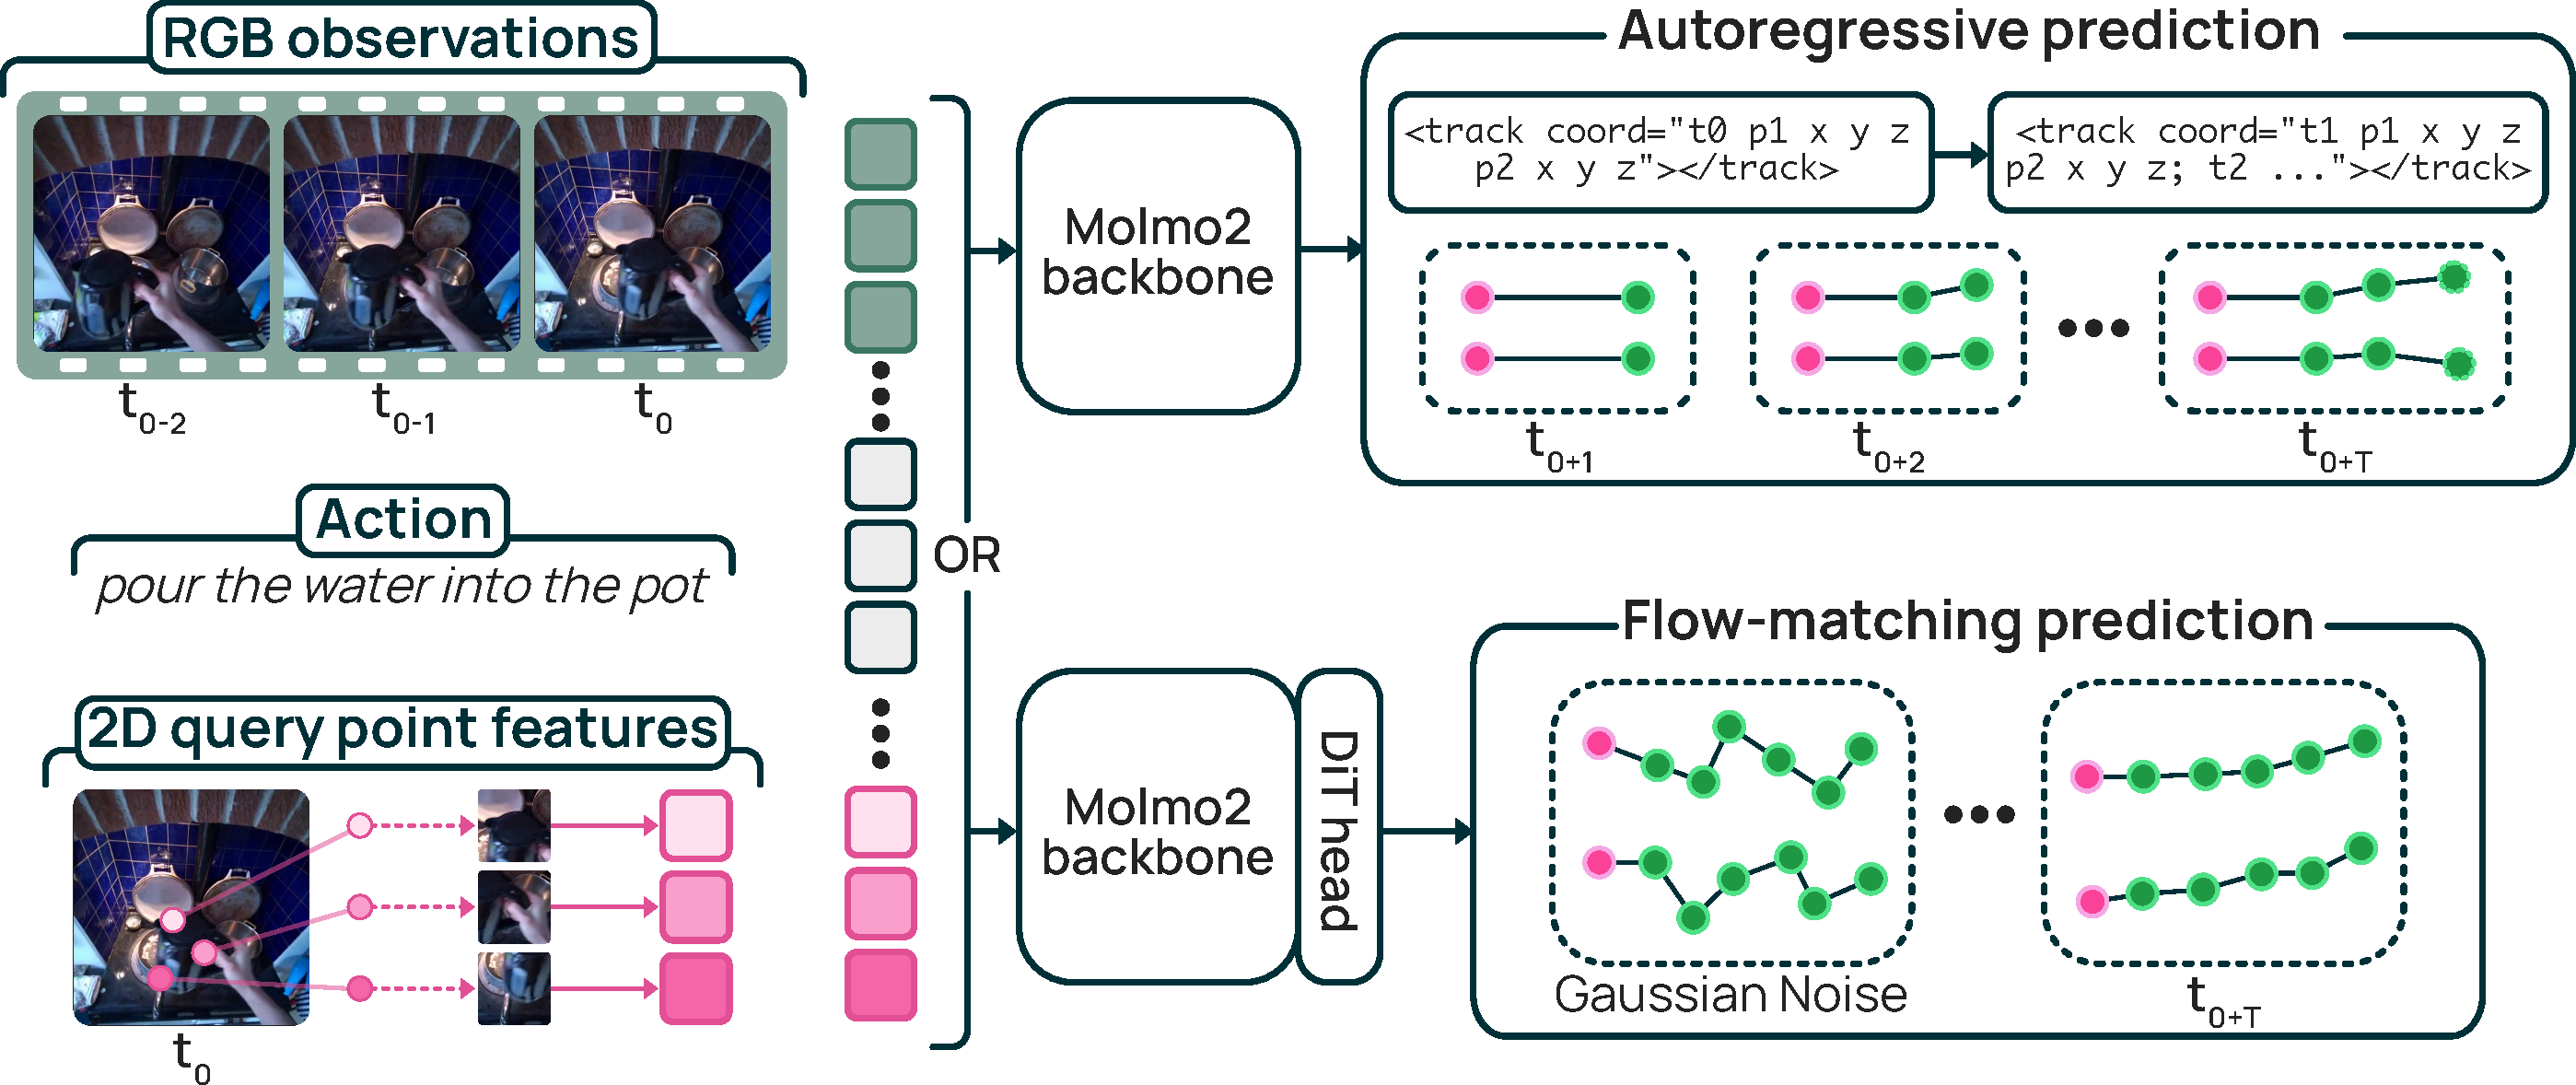
\includegraphics[width=0.93\linewidth]{figures/model_arc_4.pdf}
    \caption{\textbf{\modelname architecture.}
    The shared input to Molmo2~\cite{clark2026molmo2} backbone consists of image tokens of RGB observations, text tokens of action description, and 2D query point feature tokens sampled from Molmo2 vision encoder. 
    The autoregressive variant encodes the initial 3D query coordinates and decodes future trajectories as quantized coordinate text, while the flow-matching variant represents them directly in continuous 3D coordinate space. }
    \label{fig:architecture}
\end{figure}

\subsection{\modelname architecture}
\label{subsec:model}



We implement two classes of trajectory predictors: one with an autoregressive objective and the other with a flow-matching objective. They share the same input encoding of the RGB observation, action description, and 2D query-point visual features.
They differ in how the initial 3D query coordinates are encoded and how the future 3D trajectories are decoded (Fig.~\ref{fig:architecture}).
We study both objectives because they offer complementary modeling biases: autoregressive decoding conditions each prediction on the previously generated trajectory, which encourages smooth temporal evolution, while flow-matching models a distribution over future trajectories and is better suited for capturing motion uncertainty~\cite{chi2024diffusionpolicyvisuomotorpolicy}.

\noindent\textbf{Input encoding.}
Predicting object motion from a language instruction first requires grounding the relevant object in the image and understanding the instruction. We therefore use Molmo2~\cite{clark2026molmo2} as the vision-language backbone for input processing, leveraging its strong object-grounding capability. 
Given the RGB observation history $I_{t_s:t_0}$, the Molmo2 vision encoder produces image tokens $\mathcal{T}_{\mathrm{img}}$. The action description $a$ is tokenized into language tokens $\mathcal{T}_{\mathrm{text}}$. To condition on the query points, we additionally insert one visual point token for each 2D query coordinate. Let $F_{t_0}$ be the anchor-frame feature map produced by the vision encoder. 
For each query point $\mathbf{q}_{t_0}^{n}$, we bilinearly sample the anchor-frame feature map $F_{t_0}$ at its 2D location to obtain a point feature $\mathbf{e}_{\mathrm{pt}}^{n}$.
These features form the point-token sequence
$\mathcal{T}_{\mathrm{pt}}=\{\mathbf{e}_{\mathrm{pt}}^{1},\ldots,\mathbf{e}_{\mathrm{pt}}^{N}\}$.
We concatenate the image, text, and point tokens as
$\mathcal{C}=[\mathcal{T}_{\mathrm{img}},\mathcal{T}_{\mathrm{text}},\mathcal{T}_{\mathrm{pt}}]$
and process them with the Molmo2 language model component.

For both prediction variants, we represent 3D coordinates relative to the first query point at $t_0$. Let $\mathbf{p}_{\mathrm{anc}}=\mathbf{p}_{t_0}^{1}$ denote this anchor point. For each point $n$ and time $t$, our models represent 3d point coordinates as
$\boldsymbol{\delta}_{t}^{n}
=
\mathbf{p}_{t}^{n}-\mathbf{p}_{\mathrm{anc}}$.
All 3D point coordinates are in metric scale, in units of \textit{meter}.

\noindent\textbf{Autoregressive objective.}
The autoregressive variant follows Molmo2's coordinate representation, encoding both the initial 3D query coordinates and the future trajectory as structured text. Each anchor-relative coordinate is discretized into \textit{millimeter} bins
($\bar{\boldsymbol{\delta}}_{t}^{n}
=
\mathrm{round}\!\left(
1000\,\boldsymbol{\delta}_{t}^{n}
\right)$)
and serialized as timestamped point-coordinate tuples. Fig.~\ref{fig:architecture} shows an example of the coordinate encoding format.
The input prompt contains the visual-language conditioning $\mathcal{C}$ together with the serialized initial query coordinates $\{\bar{\boldsymbol{\delta}}_{t_0}^{n}\}_{n=1}^{N}$. The output is the serialized future trajectory $y_{1:L}$, generated in temporal order. An example of text pieces encoded and decoded can be found at Fig.~\ref{fig:architecture}.
We train the autoregressive model with the standard next-token objective.
At inference time, the model decodes the trajectory string autoregressively and the coordinates are parsed back into $\hat{\mathbf{P}}_{t_0+1:t_0+T}$. Since coordinates are emitted in temporal order, each future timestamp is conditioned on all earlier generated coordinates, giving the model a direct mechanism for modeling temporal dependence and smooth rollouts. 



\noindent\textbf{Flow-matching objective.}
The flow-matching variant predicts future trajectories in continuous 3D coordinate space. Following a MolmoBot-style design~\cite{deshpande2026molmobot}, we use a DiT decoder~\cite{peebles2023dit} conditioned on Molmo2 features from all layers, with lightweight MLPs for coordinate encoding and decoding. We concatenate the clean initial 3D query coordinates with a noised version of the future coordinates and project them into point tokens. We use RoPE along both the point and time axes to distinguish point identity and timestamp, analogous to the Multimodal RoPE used in Qwen2.5-VL~\cite{su2023roformerenhancedtransformerrotary,bai2025qwen25vl}.

The decoder is trained with the standard flow-matching objective~\cite{lipman2023flowmatching}. Specifically, we sample Gaussian noise with the same shape as the future trajectory, linearly interpolate between the noise and the ground-truth trajectory, and train the decoder to predict the corresponding velocity field from the noised trajectory to the clean trajectory. At inference time, the model starts from Gaussian noise and integrates the learned velocity field with 10 Euler steps to obtain the predicted future trajectory.



\begin{figure}[t]
    \centering
    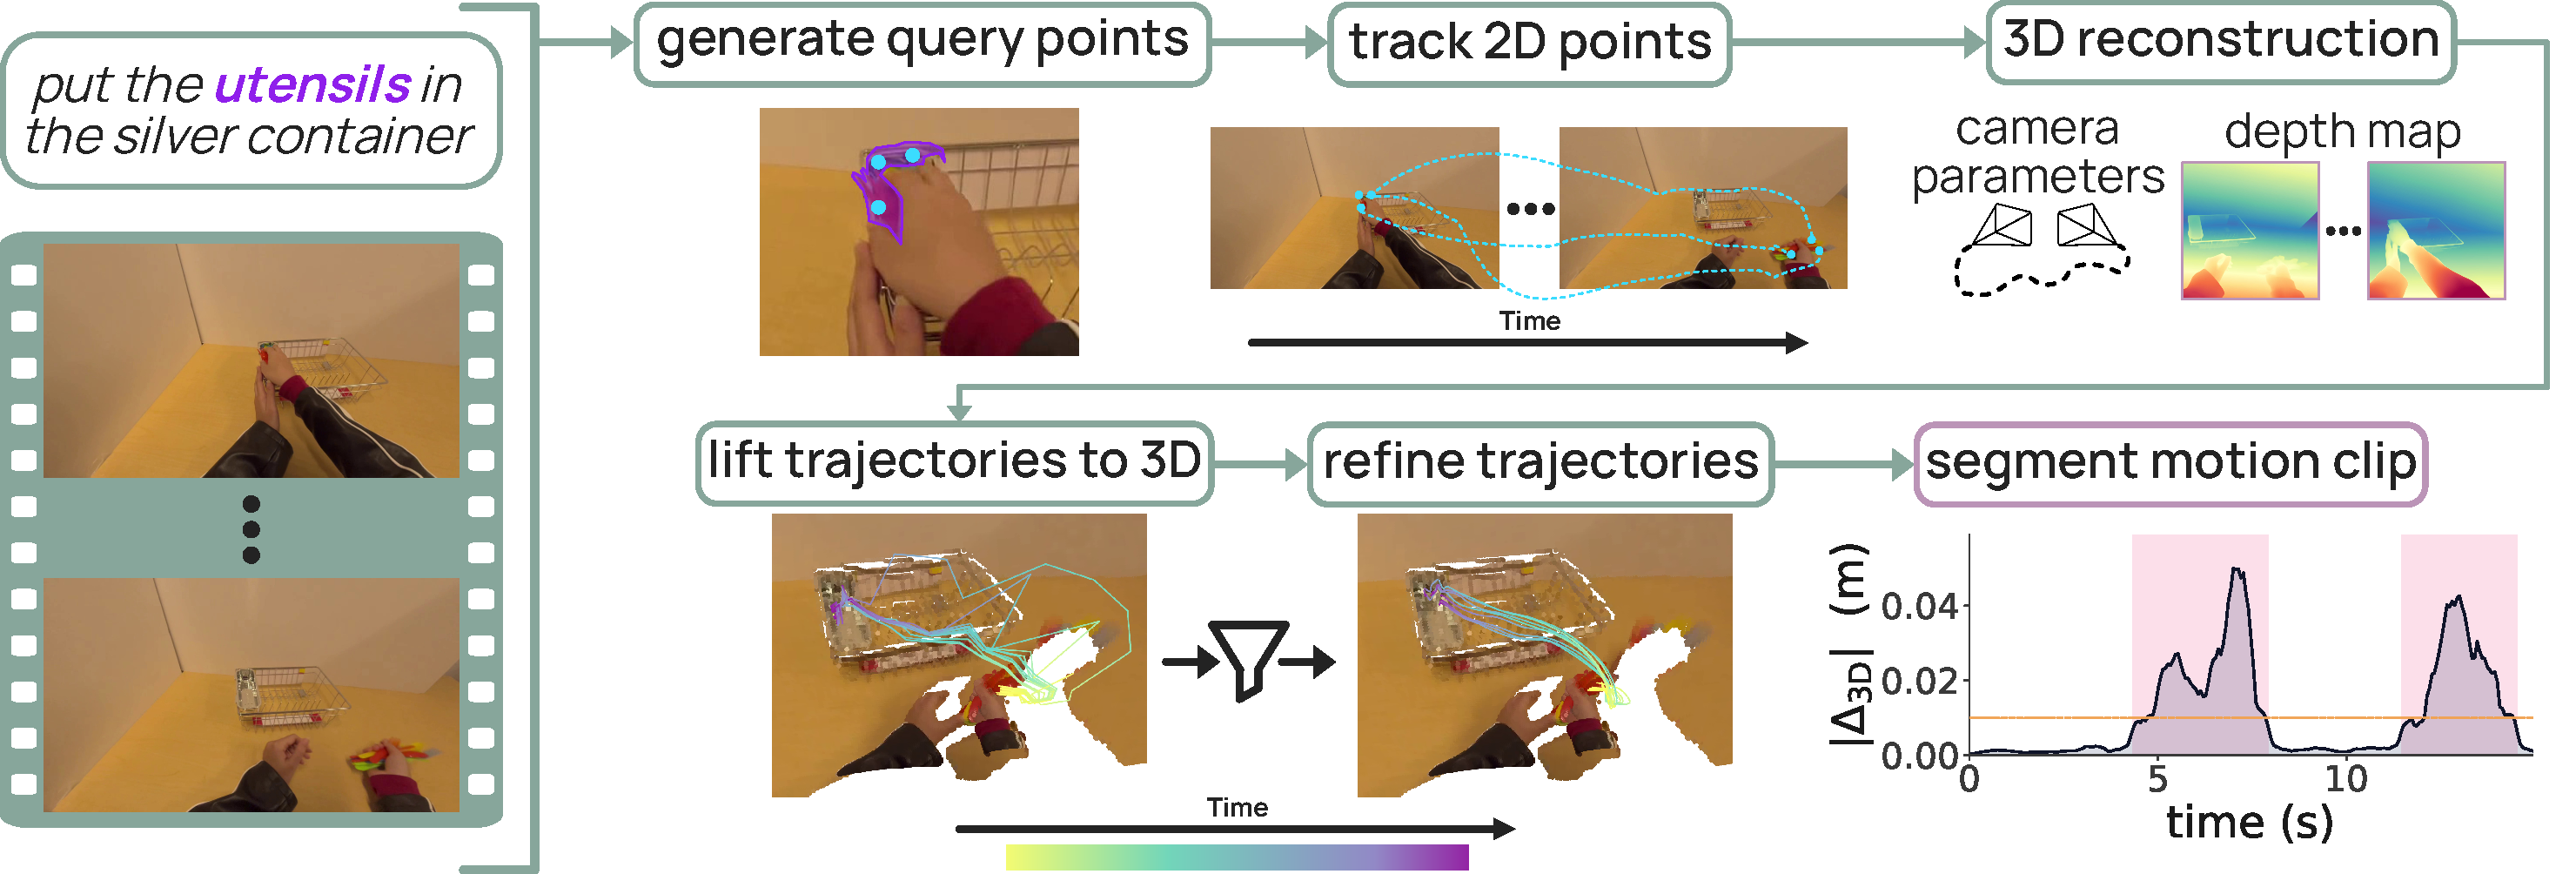
\includegraphics[width=0.93\linewidth]{figures/pipeline_3.pdf}
    \caption{\textbf{Overview of data annotation pipeline.}  Given a video of an action event and its description, we first ground the moving object and sample query points on it. We then track dense 2D points on the object, lift these tracks into a shared metric 3D frame, and use object-level spatial and temporal consistency priors to filter unreliable trajectories. Finally, we clip the video around intervals where the grounded object undergoes meaningful motion.}
    \label{fig:pipeline}
\end{figure}


\section{MolmoMotion-1M and \benchmarkname{}}



Existing 3D point-track datasets are small, domain-limited, and often lack object grounding or language annotations. We therefore build an automatic annotation pipeline that extracts object-grounded 3D point trajectories from unconstrained videos. Applying it to 1.16M public videos yields \textbf{MolmoMotion-1M}, the largest action-described, object-grounded 3D point trajectory dataset. We also introduce \textbf{\benchmarkname{}}, a held-out benchmark with verified 3D point trajectories for object-centric 3D motion forecasting.


\subsection{MolmoMotion-1M Annotation}
\label{subsec:motion_annotation}


We start with public video datasets that provide action descriptions or task captions~\cite{egodex, hdepic, xperience, stereo4d}. Our goal is to localize the described object, select query points, and track them in 3D world coordinates. The pipeline consists of five stages, shown in Fig.~\ref{fig:pipeline}: semantic object grounding, temporal point correspondence, metric 3D lifting, trajectory-level filtering, and video-level clipping.



\noindent\textbf{Semantic object grounding.}
Given an action description $a$, we use an LLM~\cite{yang2025qwen3} to extract the manipulated or moving entity as a short object phrase. Instead of prompting SAM3~\cite{sam3} to directly produce an object mask from this phrase, we first use MolmoPoint~\cite{clark2026molmopoint} to localize the entity as a 2D point in the reference frame $t_0$. We find MolmoPoint more reliable for vague phrases like ``an object on top of the table,'' because the prompt can specify the object by its action, e.g., the object being moved, rather than by appearance alone. We then use the point prompt with SAM3 to obtain the object mask $M_{t_0}$, and sample $N$ query points $\{\mathbf{q}_{t_0}^{n}\}_{n=1}^{N}$ inside $M_{t_0}$ using K-means cluster centers.

\noindent\textbf{2D point tracking and metric 3D lifting.}
We next establish point correspondence across frames by tracking the query points through the video. We run AllTracker~\cite{alltracker} to obtain temporally persistent 2D tracks  $\{\mathbf{q}_{t}^{n}\}_{t=1}^{L}$ and visibility masks $\{m_t^{n}\}_{t=1}^{L}$.
To lift these tracks into 3D, we run ViPE~\cite{vipe} on the monocular video to estimate per-frame metric depth and camera geometry. We empirically find that this paradigm produces more accurate 3D trajectories than current end-to-end 3D point trackers such as SpatialTrackerV2~\cite{spatialtrackerv2}. ViPE also provides metric scale output, allowing the resulting trajectories to be expressed in physical 3D units rather than a arbitrary relative scale.  Using the estimated depth, intrinsics, and camera poses, we back-project each visible 2D track point into a world frame anchored at the first-frame camera, producing metric 3D tracks $\{\tilde{\mathbf{p}}_{t}^{n} \in \mathbb{R}^3\}_{t=1}^{L}$.

\noindent\textbf{Trajectory-level filtering and smoothing.}
We empirically find that some lifted trajectories can be corrupted by 2D tracking drift, depth noise, and camera estimation errors. 
We therefore both filter outlier tracks and smooth remaining tracks using the object-level prior that sampled points should move coherently as parts of the same physical entity.
We remove tracks with consistently low trust using a MAD-based outlier criterion~\cite{leys2013madoutlier}.
For retained tracks, we follow the smoothing algorithm in Stereo4D~\cite{stereo4d} to smooth their depth value along each camera ray. More details can be found in Appendix~\ref{appsec:filtering}.
This removes high-frequency depth jitter in annotated 3D tracks.

\noindent\textbf{Video-level clipping.}
Event-level video clips often contain long static intervals before or after the described motion, which provide little supervision for learning dynamics. We therefore re-clip videos around intervals where the grounded object actually moves.
Given the filtered 3D trajectories, we compute a per-frame object motion score $s_t$ as the median 3D displacement of valid object points:
$
s_t
=
\mathrm{median}_{n}
\left\|
\mathbf{p}_{t}^{n}
-
\mathbf{p}_{t-1}^{n}
\right\|_2 .
$
We threshold $s_t$ to obtain contiguous segments with non-trivial object motion. This step also automatically removes static videos.




\begin{figure}[t]
\centering
\begin{subfigure}{0.32\linewidth}
    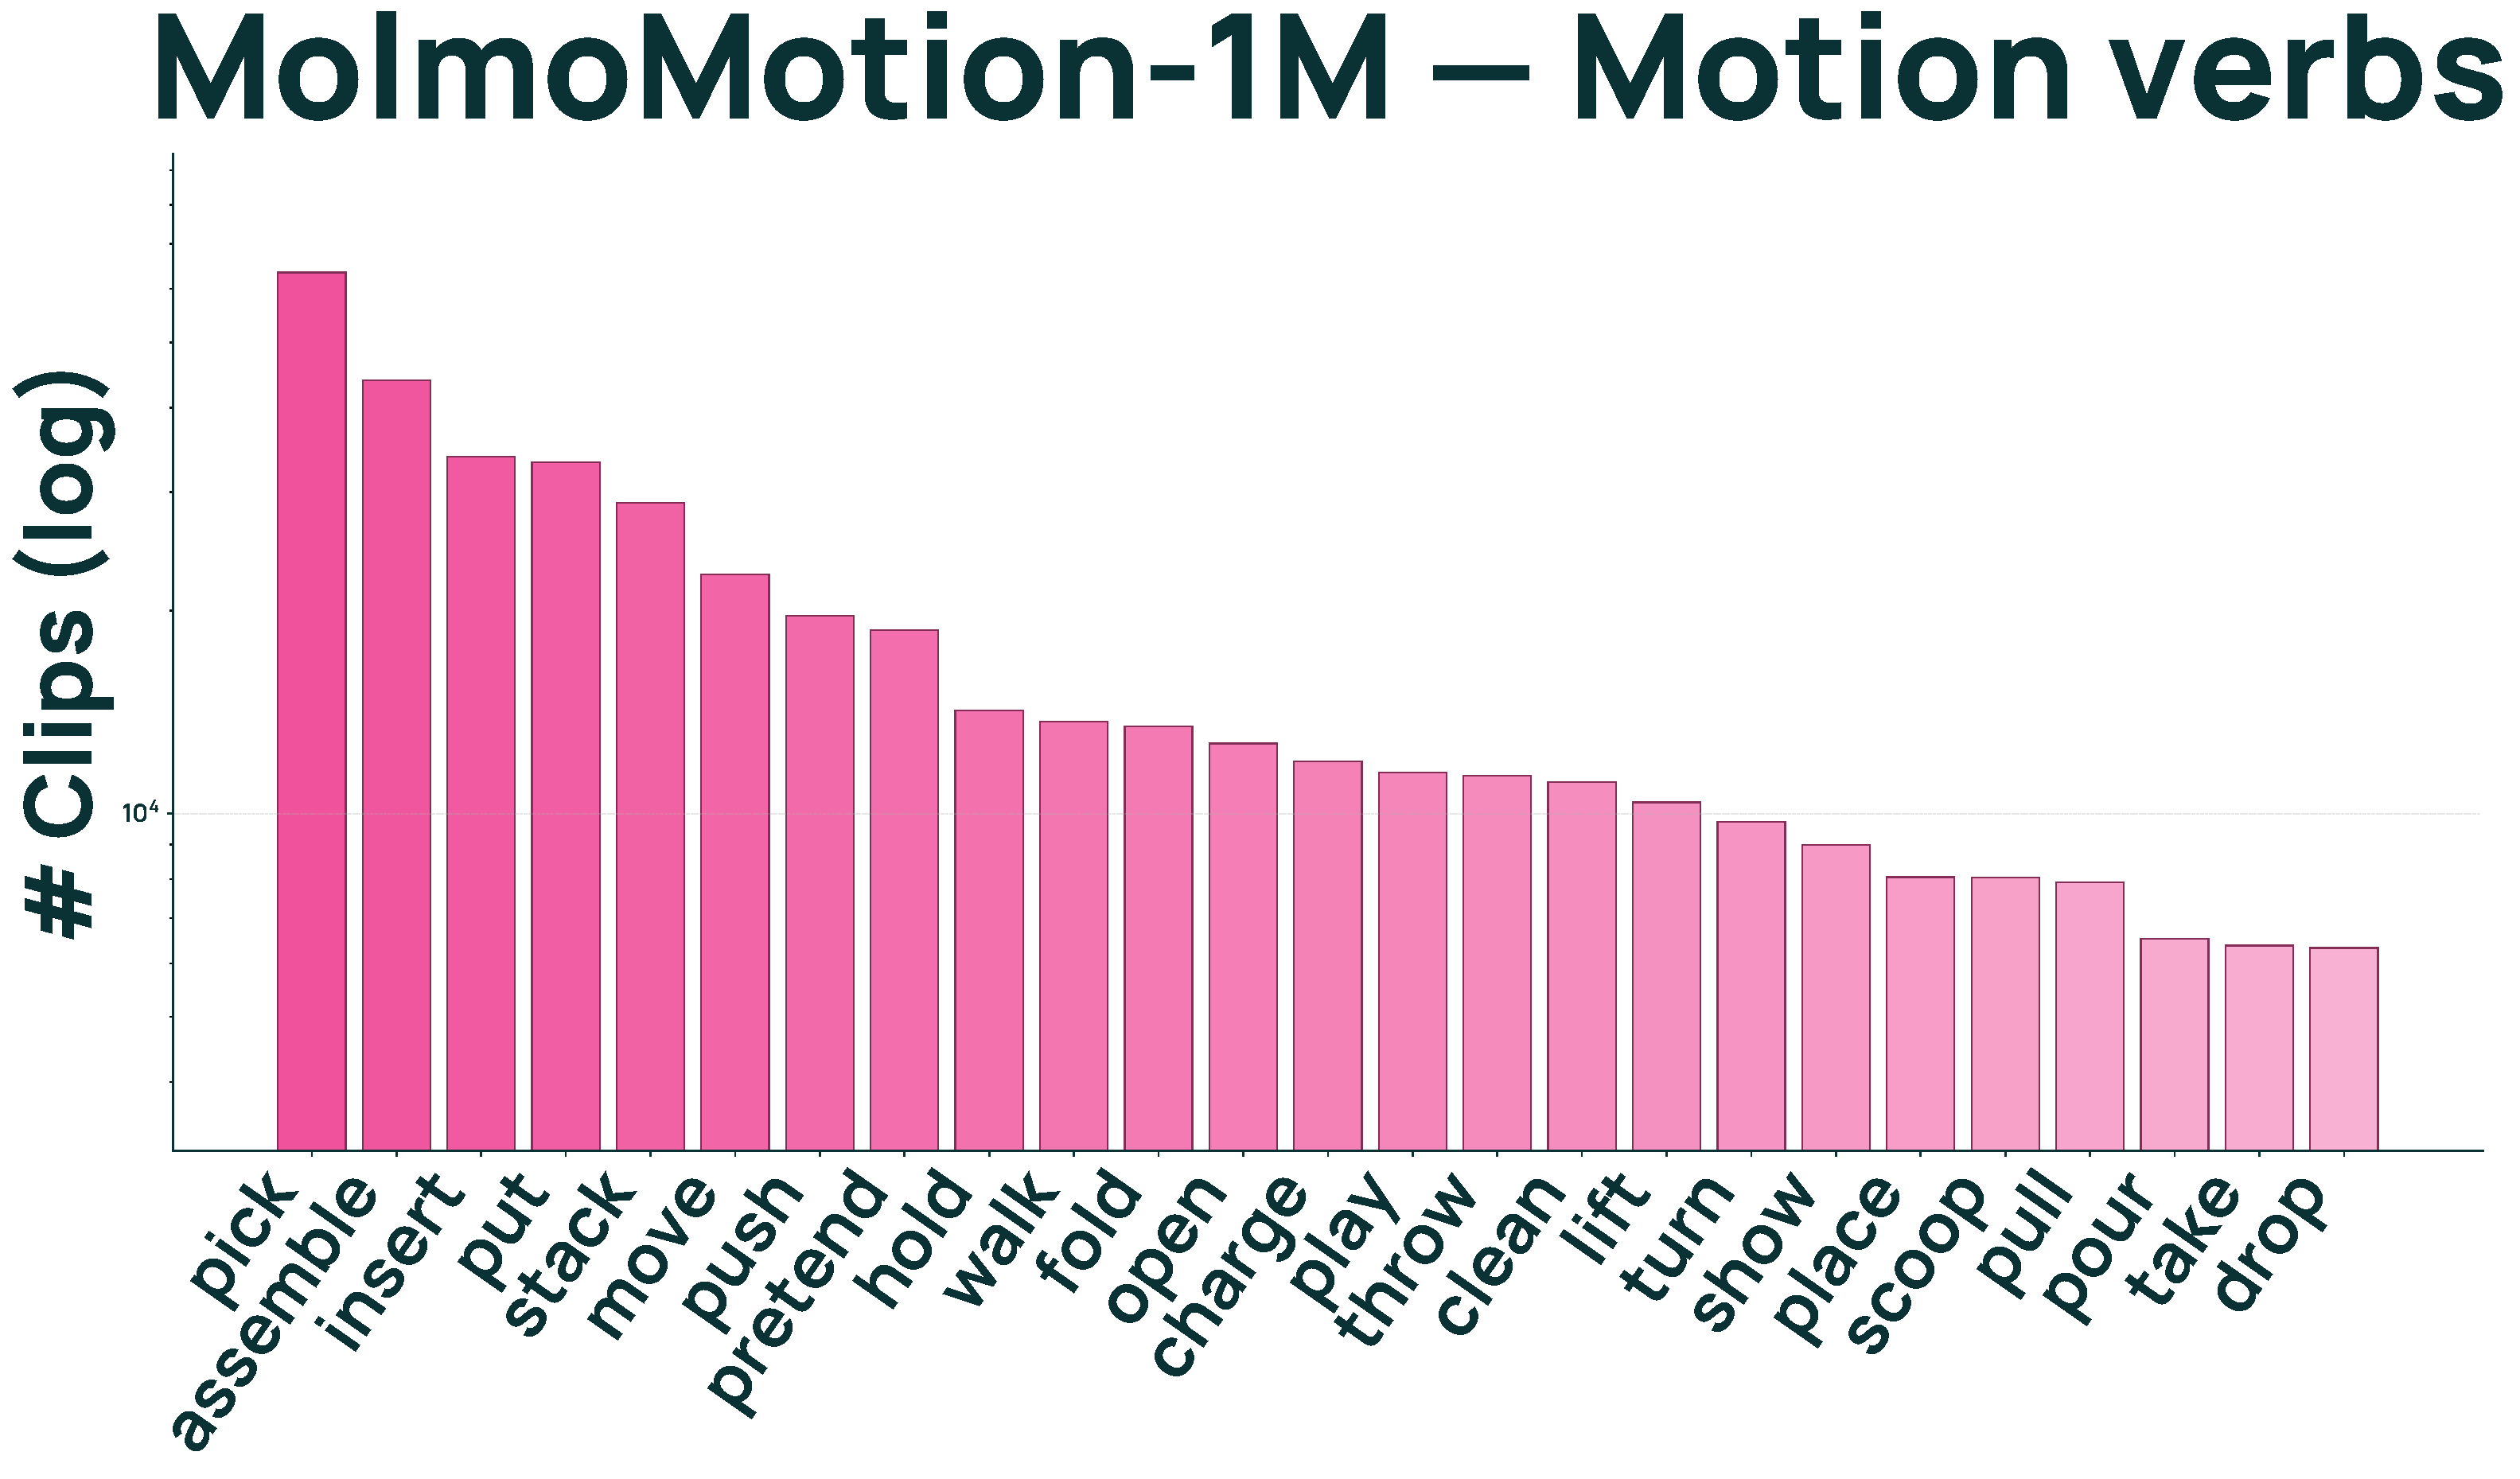
\includegraphics[width=\linewidth]{figures/verbs_pretrain.pdf}
    \caption{MolmoMotion-1M (pretrain).}
\end{subfigure}\hfill
\begin{subfigure}{0.32\linewidth}
    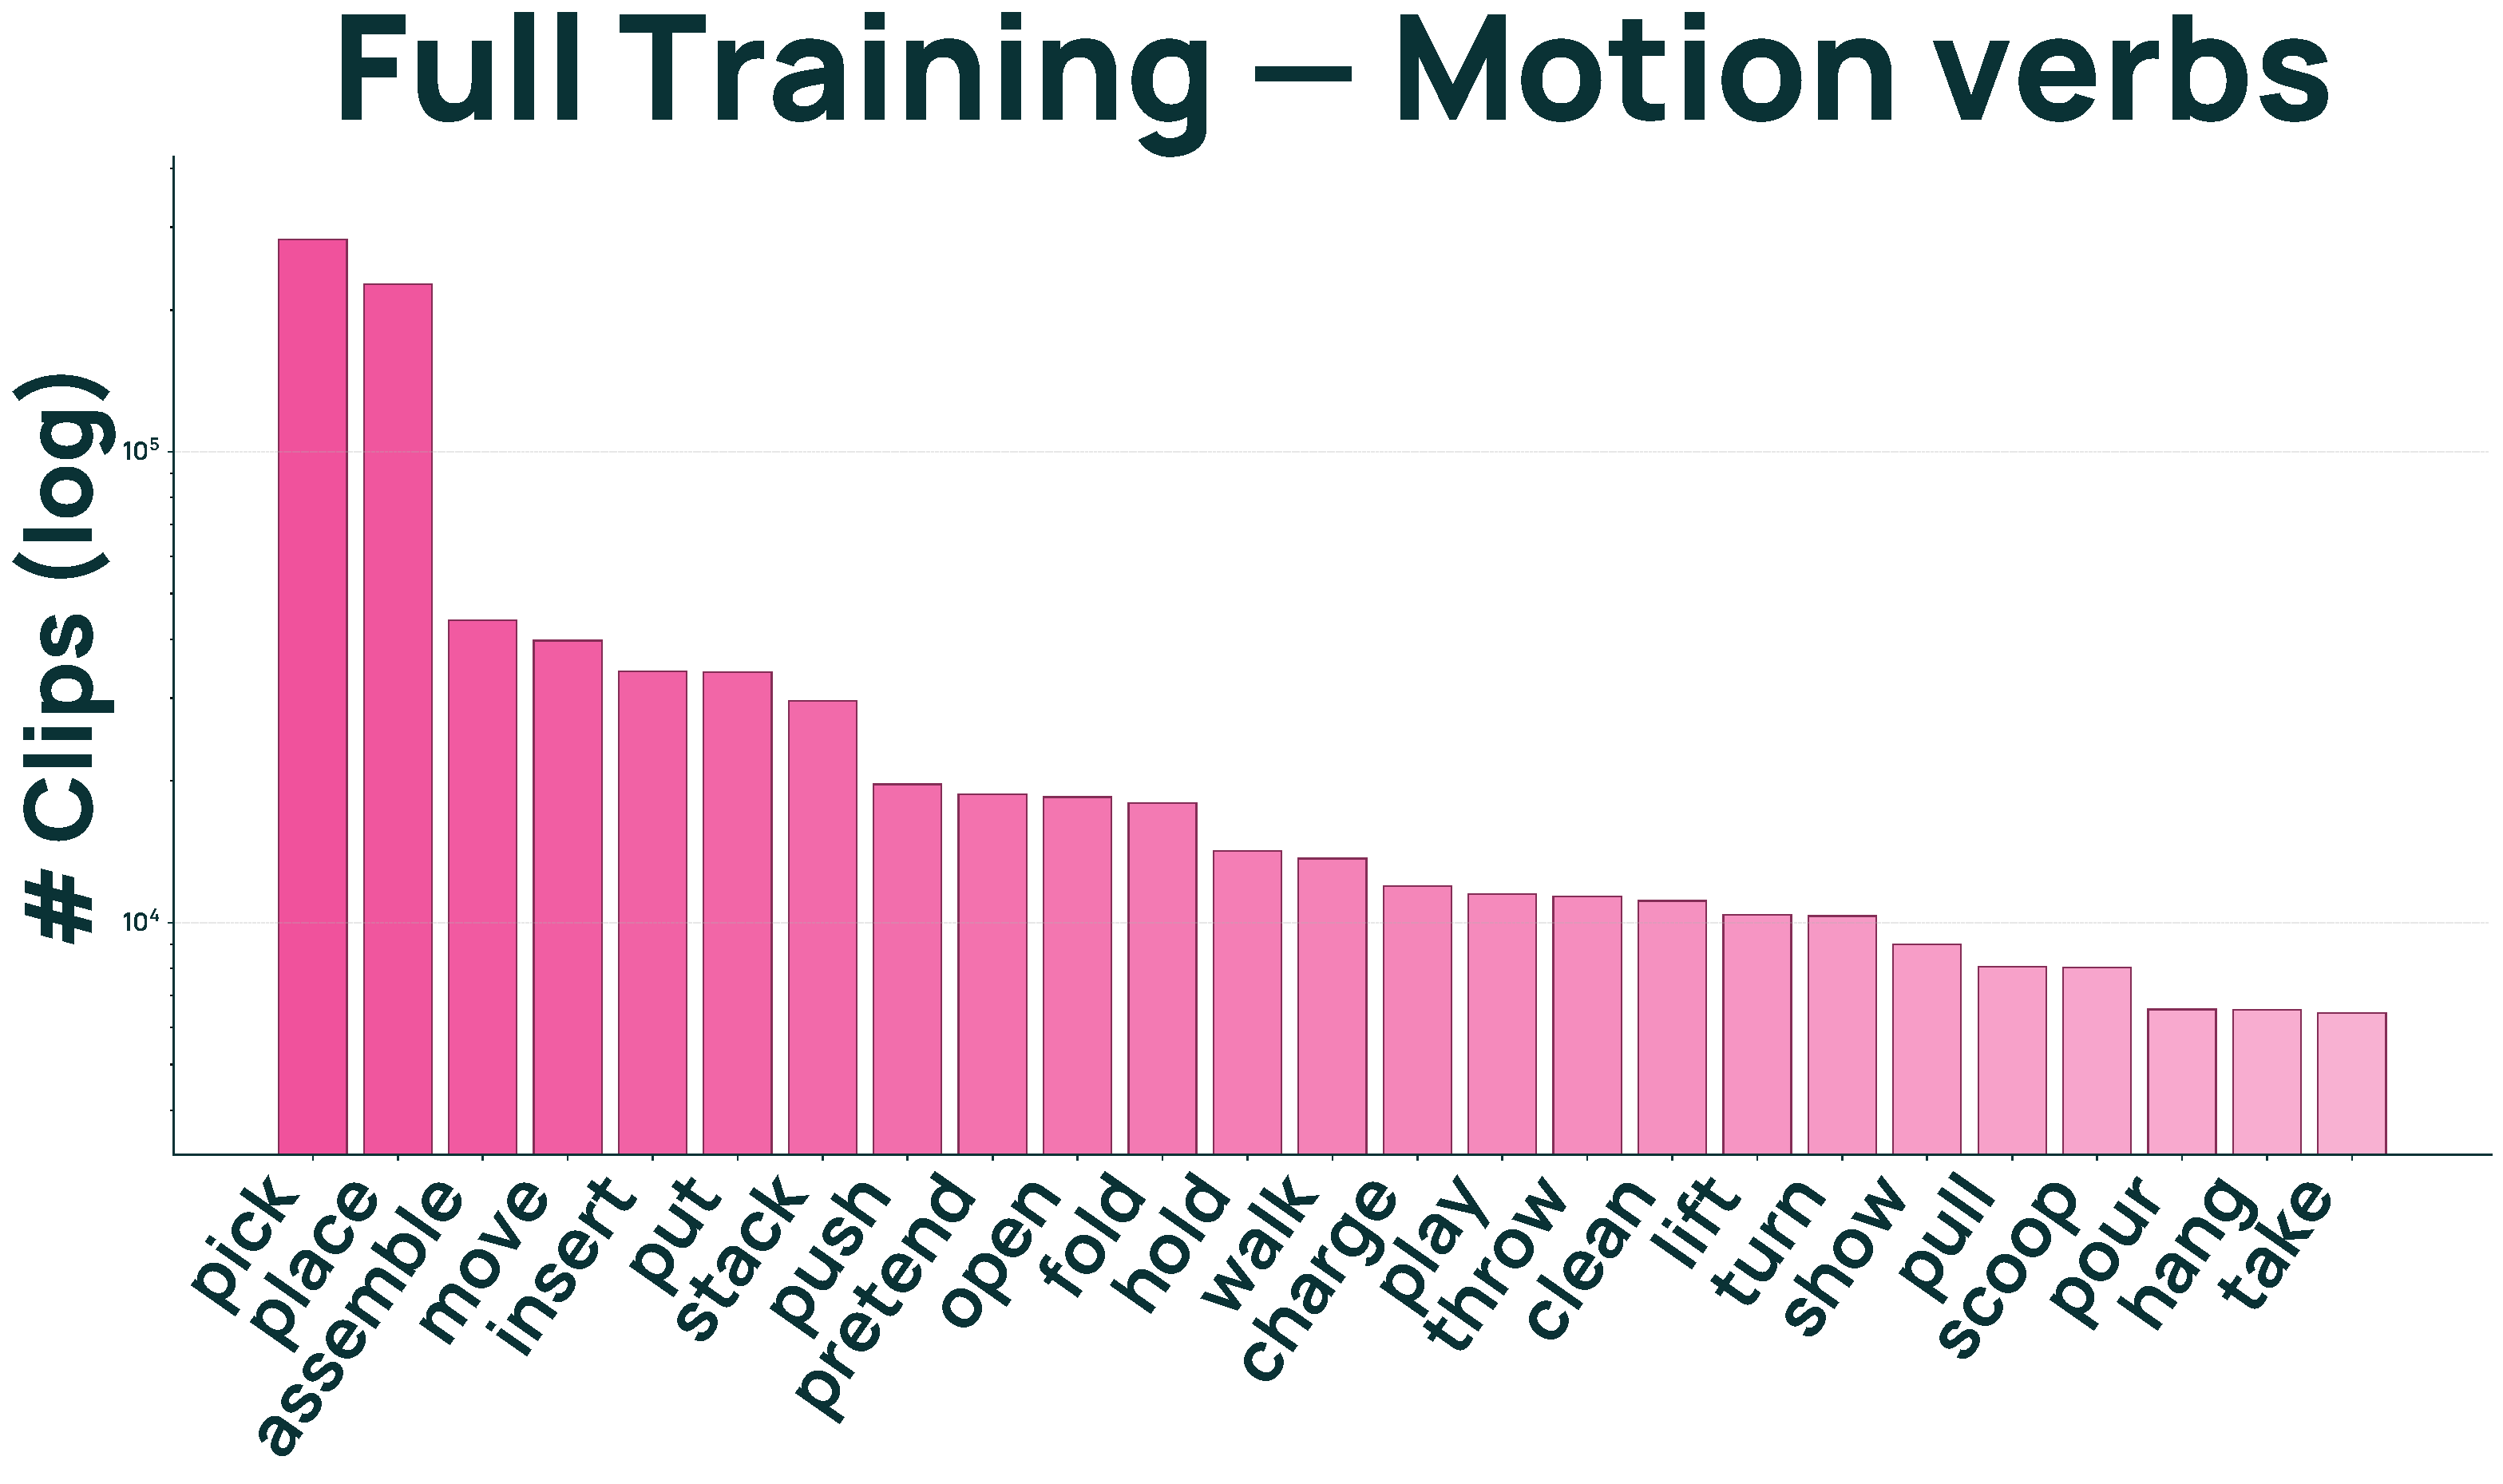
\includegraphics[width=\linewidth]{figures/verbs_fulltrain.pdf}
    \caption{Pretrain + downstream.}
\end{subfigure}\hfill
\begin{subfigure}{0.32\linewidth}
    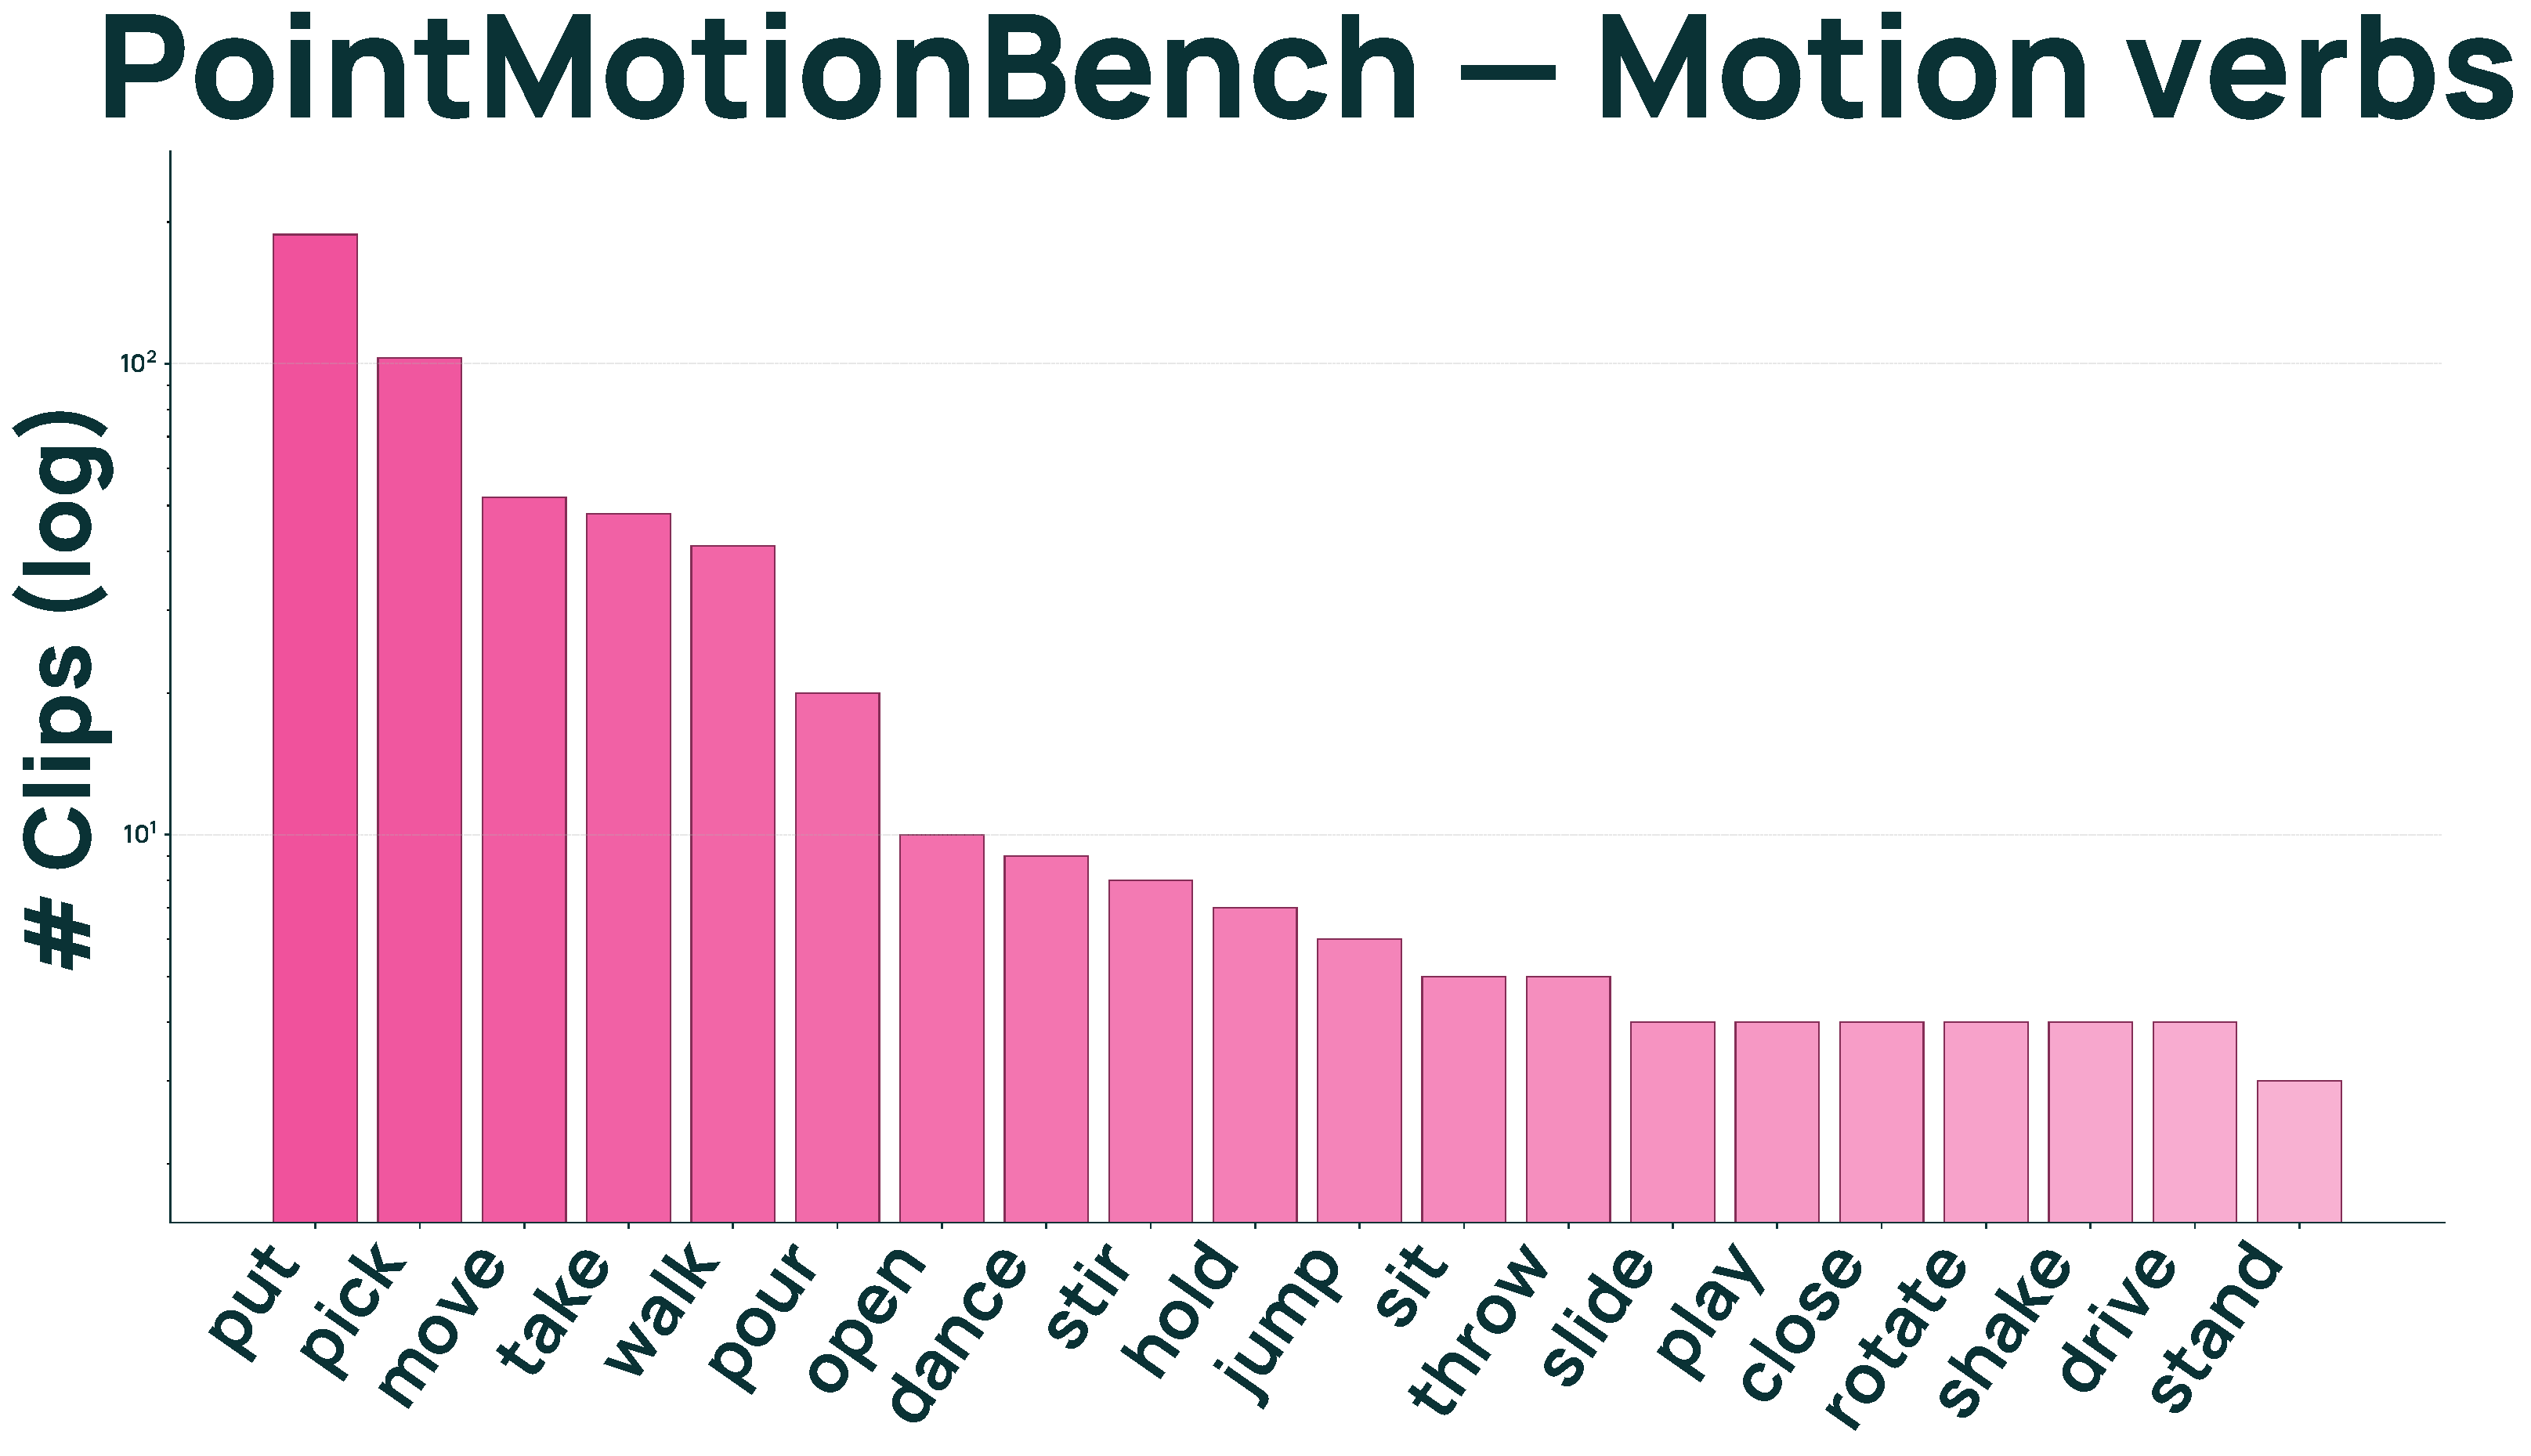
\includegraphics[width=\linewidth]{figures/verbs_bench.pdf}
    \caption{\benchmarkname{}.}
\end{subfigure}
\caption{\textbf{Action-verb diversity.} Distribution of the most frequent motion verbs across the pretraining corpus (MolmoMotion-1M), the full training corpus that additionally includes the MolmoSpaces and DROID downstream-finetune data, and the \benchmarkname{} evaluation set. Bars are log-scaled.}
\label{fig:diversity-verbs}
\end{figure}

\begin{figure}[t]
\centering
\begin{subfigure}{0.32\linewidth}
    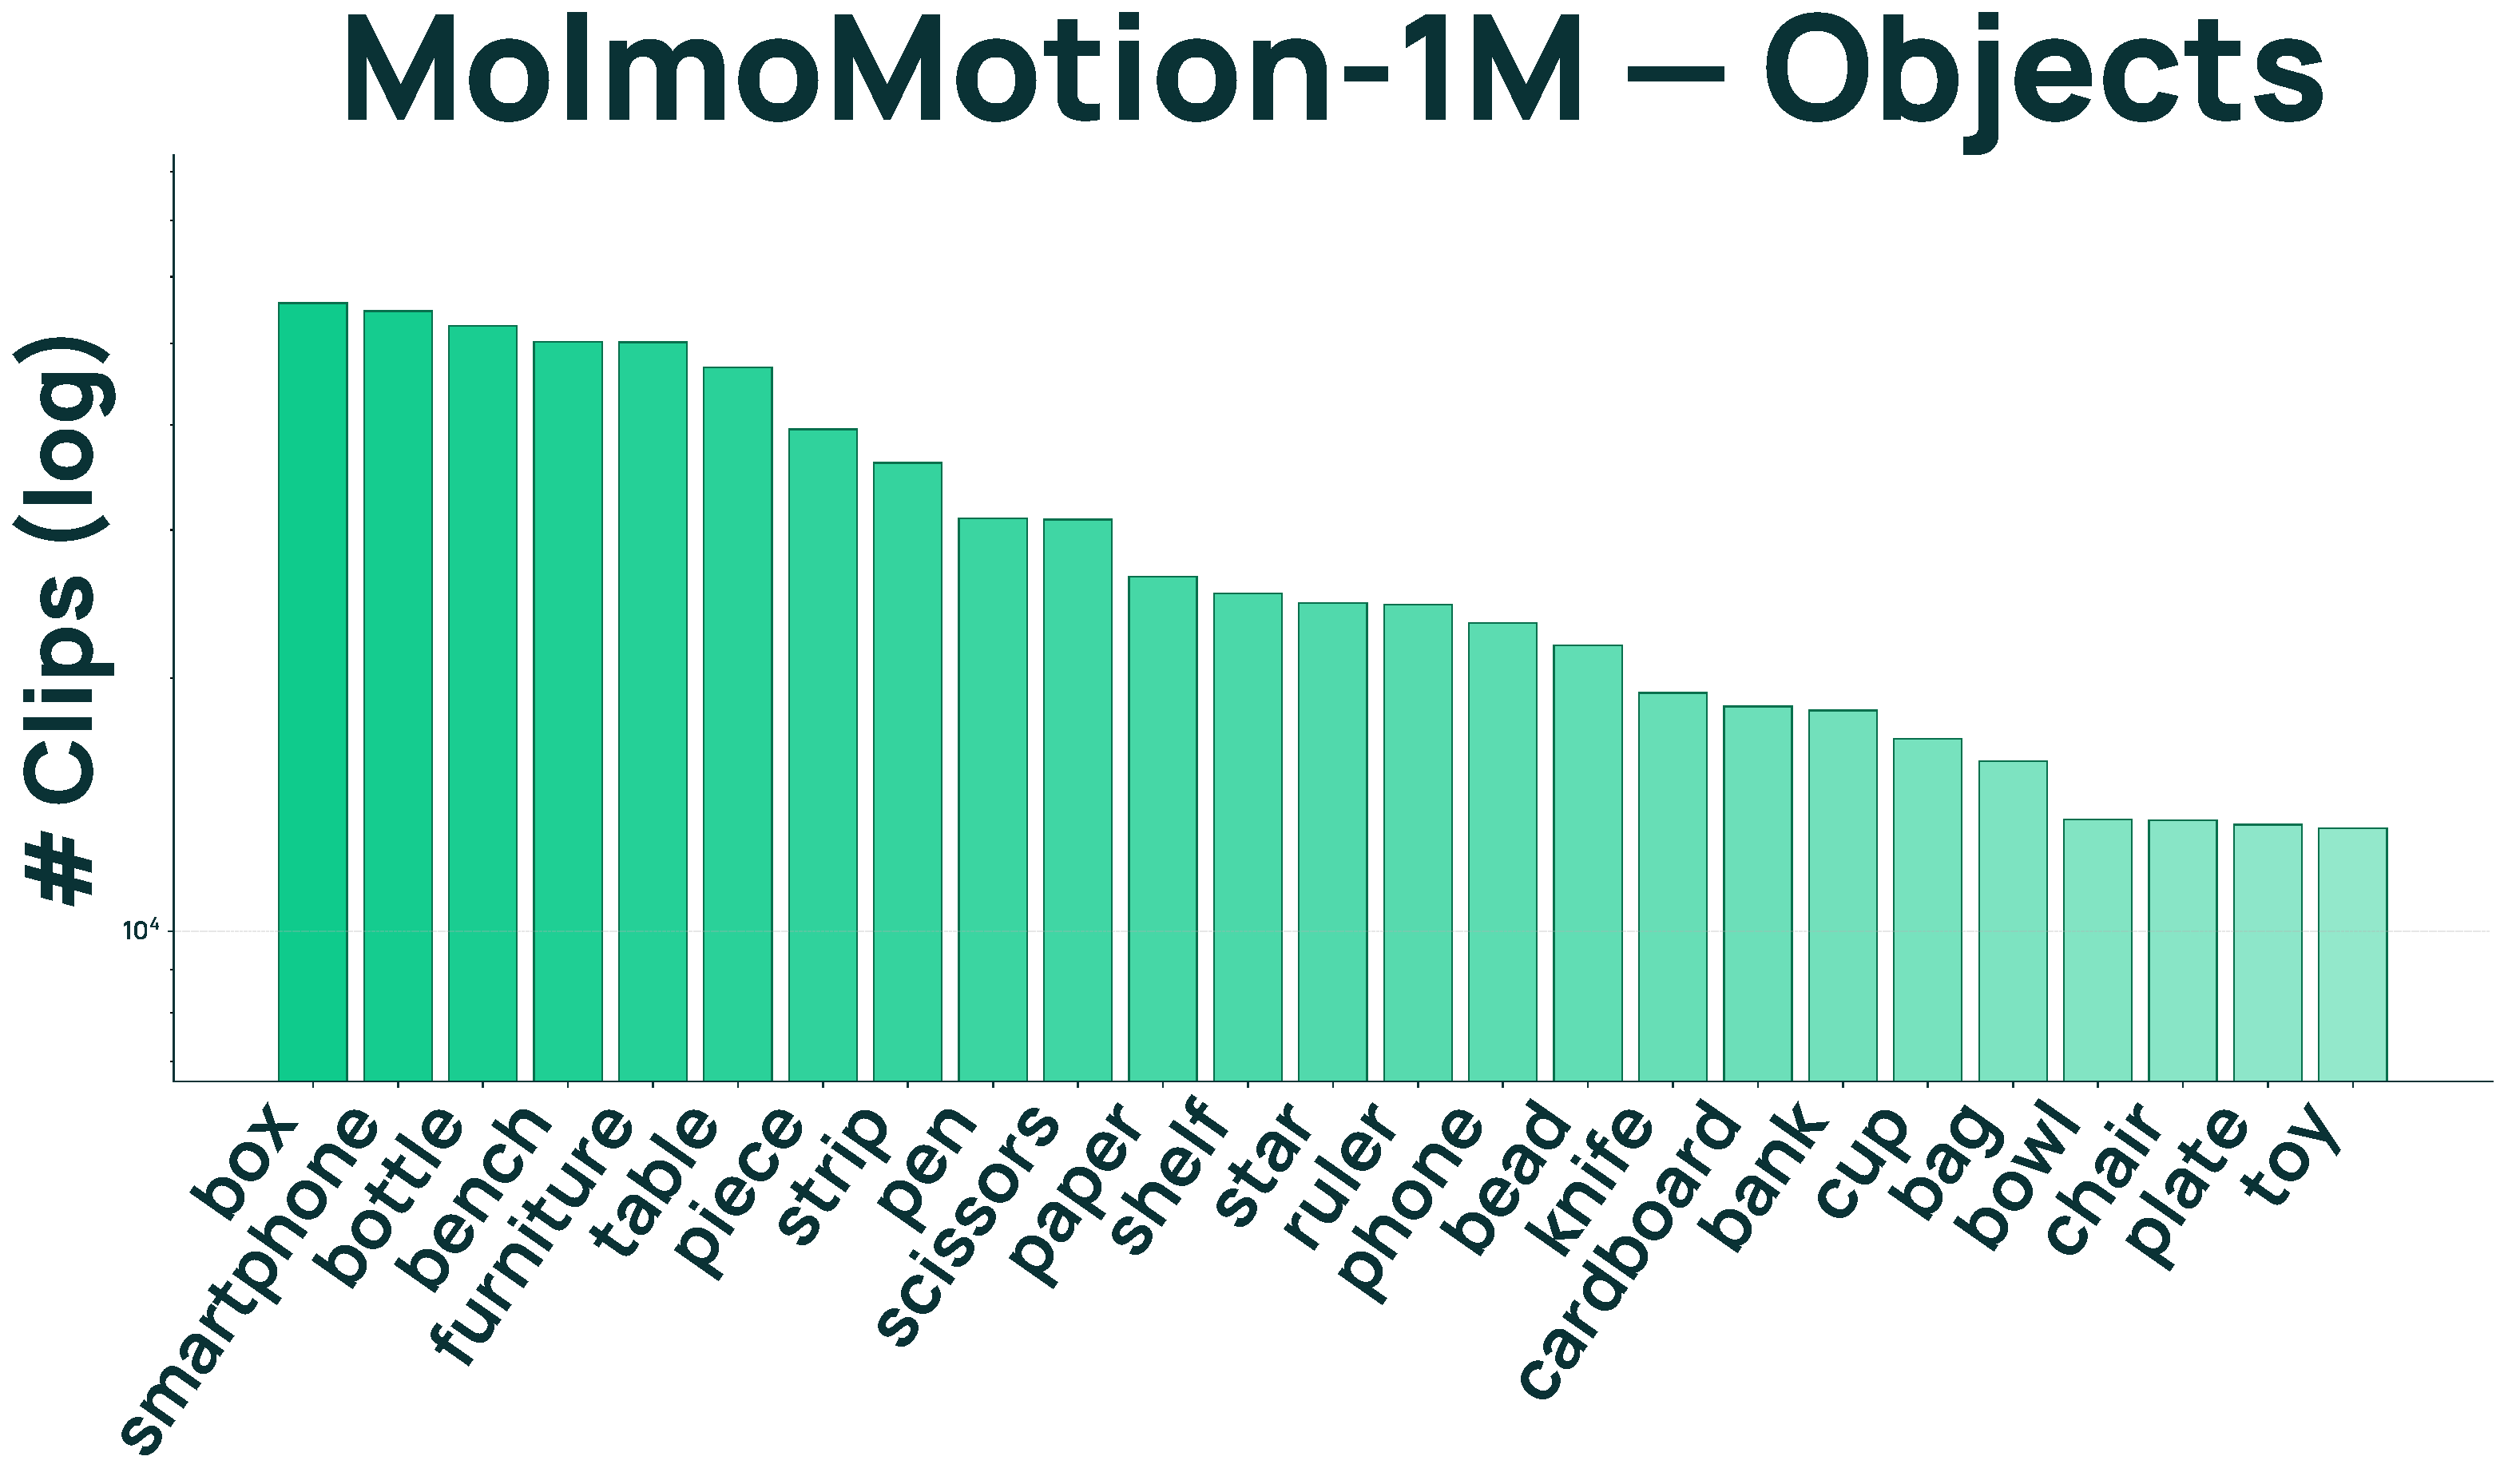
\includegraphics[width=\linewidth]{figures/objects_pretrain.pdf}
    \caption{MolmoMotion-1M (pretrain).}
\end{subfigure}\hfill
\begin{subfigure}{0.32\linewidth}
    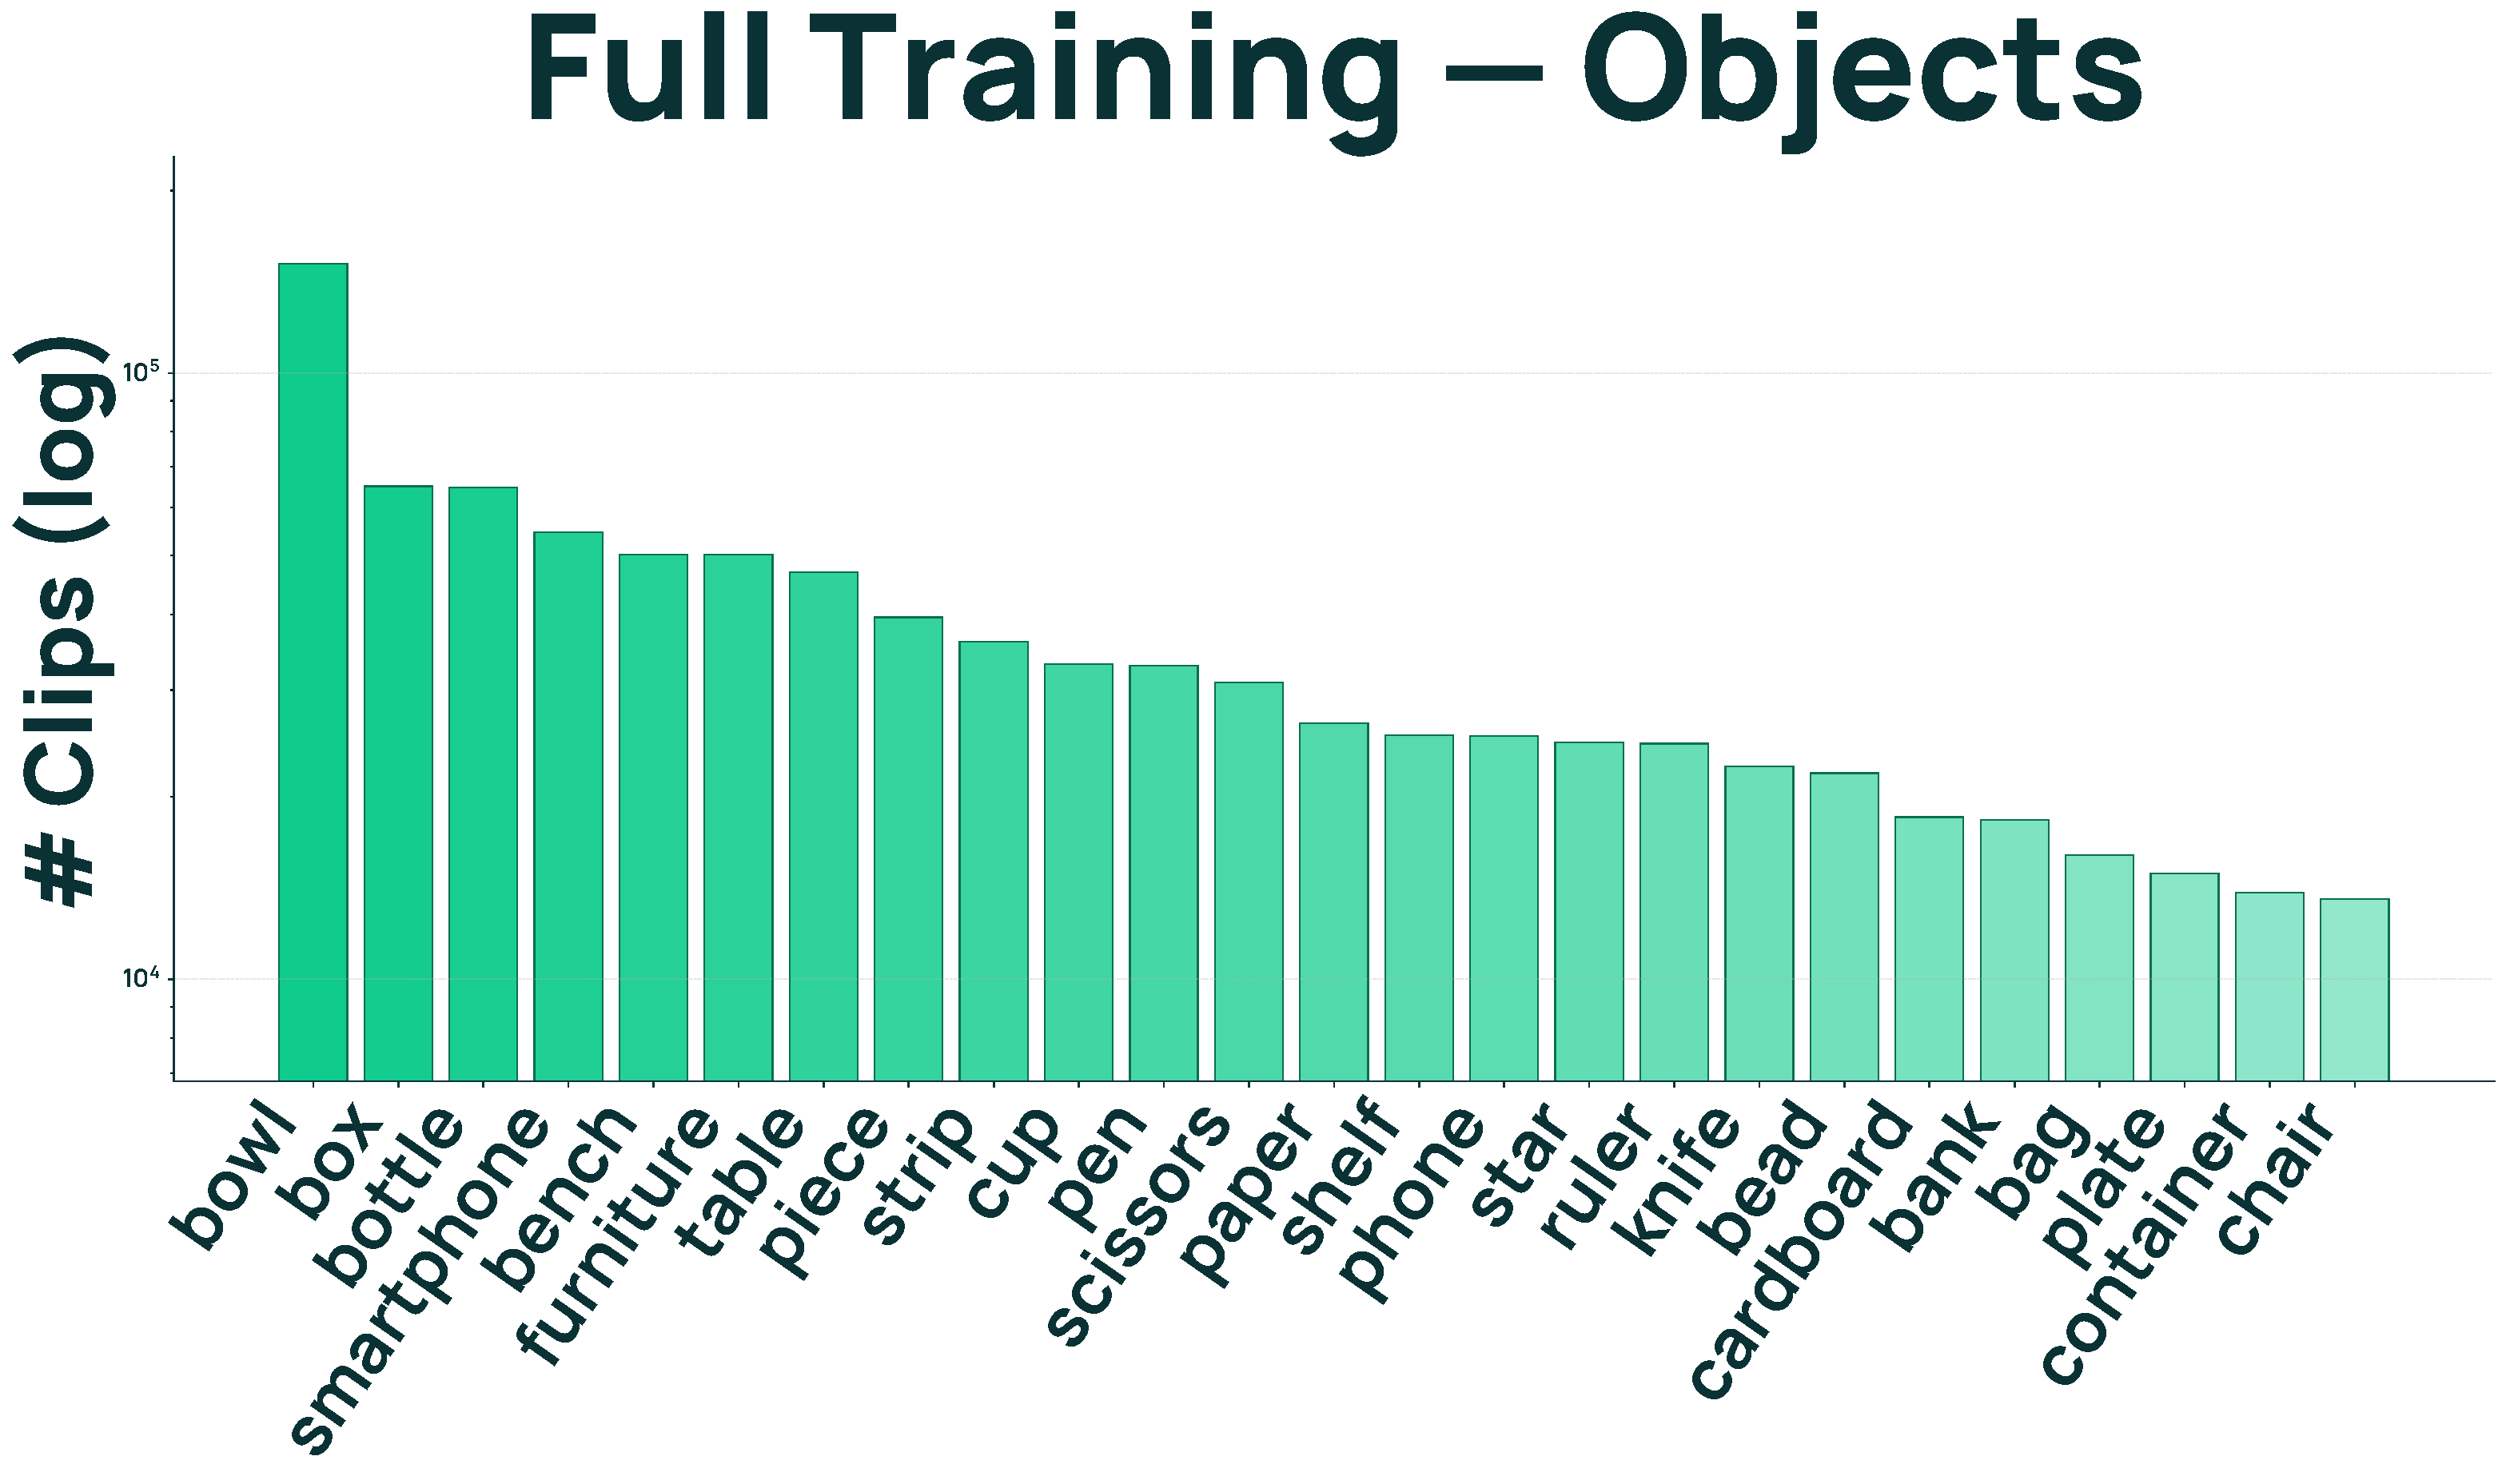
\includegraphics[width=\linewidth]{figures/objects_fulltrain.pdf}
    \caption{Pretrain + downstream.}
\end{subfigure}\hfill
\begin{subfigure}{0.32\linewidth}
    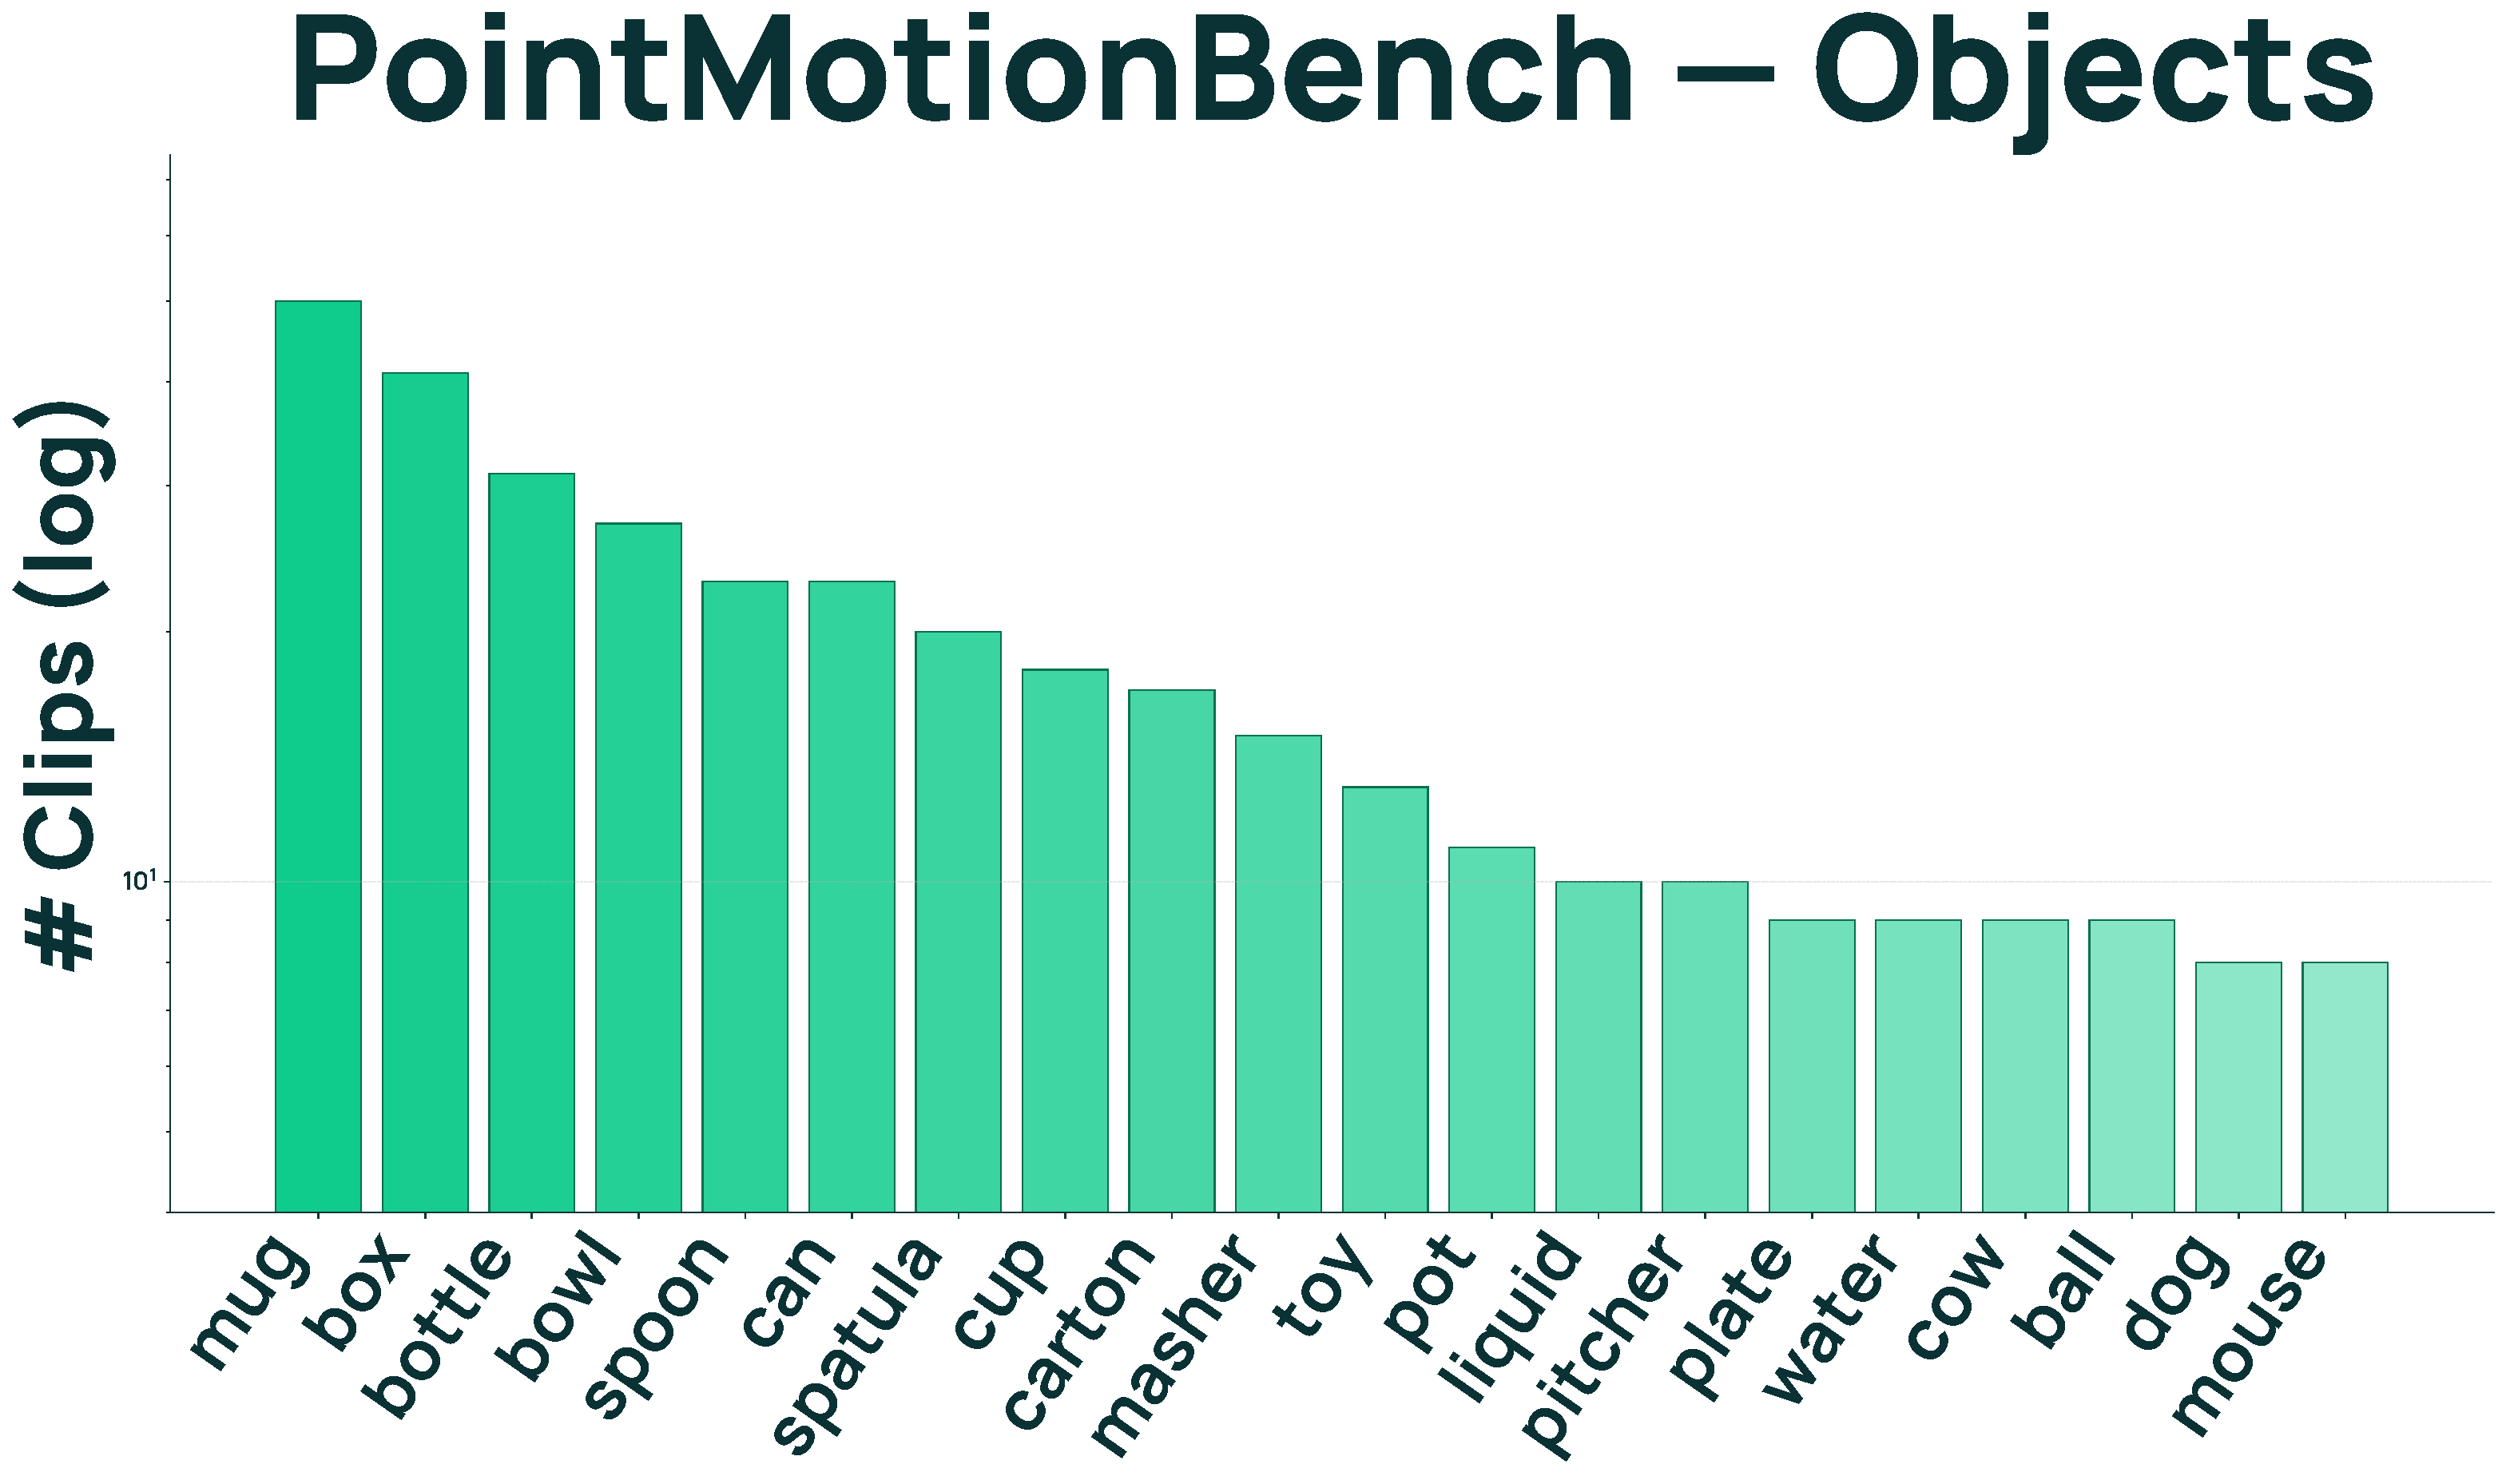
\includegraphics[width=\linewidth]{figures/objects_bench.pdf}
    \caption{\benchmarkname{}.}
\end{subfigure}
\caption{\textbf{Manipulated-object diversity.} Distribution of the most frequent manipulated objects per cohort. Generic placeholder tokens (\textit{object}, \textit{hand}, \textit{person}) are excluded. Bars are log-scaled.}
\label{fig:diversity-objects}
\end{figure}


\noindent\textbf{Pretraining corpus statistics.}
Our videos span human manipulation, hand-object interaction, and in-the-wild scenarios. The largest portion comes from human-object manipulation datasets: EgoDex~\cite{egodex}, HD-EPIC~\cite{hdepic}, and Xperience-10M~\cite{xperience} together contribute the bulk of egocentric and third-person manipulation clips; we additionally include YT-VIS~\cite{ytvis} and Stereo4D~\cite{stereo4d} clips, which broaden coverage to outdoor scenes and deformable objects like animals. 

After filtering and segmentation, the pipeline produces approximately $1$M clips with motion (per-corpus counts in Tab.~\ref{tab:appendix-sources}). The corpus spans $736$ unique action verbs and $5{,}692$ unique manipulated objects. Clips are short by construction: median clip length is $0.8$--$1.1$\,s on the manipulation corpora and $1.7$\,s on Stereo4D, where third-person walking subjects yield longer motion windows. Median per-clip 3D displacement ranges from $7$--$9$\,cm on the manipulation corpora to $51$\,cm on Stereo4D, reflecting the difference between tabletop manipulation and walking subjects. After filtering, each clip retains a median of $88$ query points (range $60$--$100$). Fig.~\ref{fig:diversity-verbs} and Fig.~\ref{fig:diversity-objects} show the per-cohort distributions of motion verbs and manipulated objects across the pretraining corpus (MolmoMotion-1M), and the full training corpus that additionally includes the MolmoSpaces and DROID data used for downstream robot finetuning.




\subsection{\benchmarkname{}}
\label{subsec:data_and_benchmark}
We also introduce \textbf{\benchmarkname{}}, a held-out benchmark for evaluating object-centric 3D motion forecasting. Unlike the pretraining corpus, which starts from videos with action descriptions, \benchmarkname{} repurposes datasets with ground-truth 3D capture to ensure annotation accuracy. For HOT3D~\cite{hot3d} and WorldTrack~\cite{feng2025st4rtrack}, we extract 3D point trajectories directly from the provided 3D object mesh or points, ground the foreground points to objects, and annotate action descriptions, with all annotations verified by humans (details in Appendix~\ref{subsec:appendix_3dworldbench}). Since HOT3D and WorldTrack mainly cover indoor manipulation and egocentric hand-object interaction, we further include DAVIS~\cite{davis} to cover outdoor dynamic scenes; for this split, we run our annotation pipeline and manually verify the correctness of each resulting trajectory.
In total, the benchmark contains $\mathbf{742}$ clips spanning $\mathbf{111}$ object categories and $\mathbf{61}$ action/motion types. Fig.~\ref{fig:diversity-verbs}(c) and Fig.~\ref{fig:diversity-objects}(c) show the per-cohort distributions of motion verbs and manipulated objects across \benchmarkname{}.
